\documentclass[a0v]{btrpstr}

\usepackage{fontspec}
\setmainfont{FiraSansLight}[
  ItalicFont=FiraSansLightItalic,
  BoldFont=FiraSansBold,
  BoldItalicFont=FiraSansBoldItalic]
\setmonofont{FiraMono}

% we will position some stuff manually
\usetikzlibrary{positioning}

% this is for the demo plot
\usepackage{pgfplots}

% sample text
\usepackage{lipsum}

\begin{document}
\begin{poster}[fontsizes=44pt]
\posterbackground{fill=black!5}

% You can draw normal nodes as with tikz.
% (poster) node is an alias for current page.
% Let's simulate a bit of a logo.
\node[anchor=north east, inner sep=1cm]
  (logo) at (poster.north east)
  {\resizebox{10cm}{!}{$\alpha\choose\omega$}};

% Make a _column_ (a vertical series of boxes with text reasonably aligned).
% Columns have names; there are functions to easily put boxes below each other
% in the columns.
\newpostercol{title}{start=(poster.north west), span=(logo.west)}

% Now let's make a box in that column
\begin{posterbox}{titlebox}{col=title,sep=.75in}
  \centering
  {\LARGE\bfseries A better \LaTeX{} poster template, now with Ti{\it k}Z features
   and a~bit of support for really long headings}

  {\large Author First, Second Author
   \quad \tt \{author,second\}@insti.tute.tld}

  Department of Poster Engineering, Great University, City
\end{posterbox}

% \splitpostercol creates a series of columns next to each other, with some
% padding, etc. Results from splitting the column 'text' will be called
% 'text1', 'text2', etc. You can specify the "parent" column spec; that will
% just create a new column 'text'.
\splitpostercol{text}{
  make parent={start=(poster.west |- titlebox.south), span=(poster.east)},
  n=2,
  side sep=2em,
  col sep=2em}

% a styled box
\begin{posterbox}{stickynote}{col=text1,style={color=yellow!50!orange!80!black, fill=yellow!25},sep=2em}
  \Large This is the main message of the whole poster!
  \bfseries Looks like a sticky note!
\end{posterbox}

% a slightly more regular box
\begin{posterbox}{whitebox}{col=text1, below=stickynote, style={fill=white}, offset=1ex}
  \lipsum[1][1-4]
\end{posterbox}

% a box with autoformatted header
% (use PGF styles to avoid writing the styles all over again!)
\begin{headerbox}{rightbox}{col=text2, header style={fill=cyan!20!black, text=white}, body style={fill=cyan!20}, header={A box, now with a header}}
  \lipsum[2]
\end{headerbox}

% now make a huge leader message (in plain tikz)
\node[text width=.8\paperwidth,text=white,font=\fontsize{6cm}{6cm}\selectfont]
  (leader) at (poster.center)
  {This really helps a lot with the design of the \textbf{\#betterposter}s.};
\node[below=of leader.south east,anchor=north east,color=white]
  (note) {\textit{--- a compendium of \TeX{}nicians, 2020}};

% make a background (a shortcut for a background node that fits everything in
% the second argument)
\posterboxbackground{leaderbg}
  {(leader)(note)(leader-|poster.west)(leader-|poster.east)}
  {inner sep=10cm,shade,top color=violet!50!black,bottom color=black}

% continue with plain text below the leader message
\begin{posterbox}{bgtest}{col=text1, below=leaderbg, offset=3cm}
  \lipsum[1][4-6]

  \vspace{2ex}
  \centering
  \pgfplotsset{width=0.5\linewidth}
  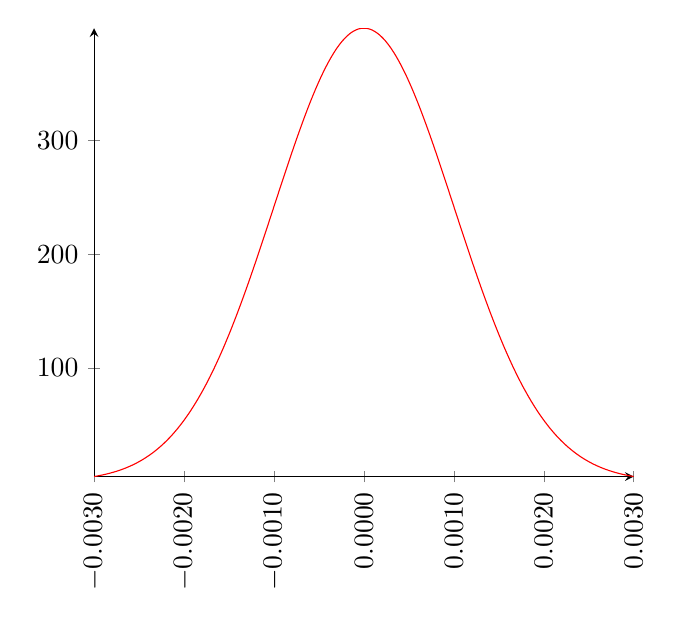
\begin{tikzpicture}
  \begin{axis}[axis lines=left, scaled ticks=false, xticklabel style={ rotate=90, anchor=east, /pgf/number format/precision=4, /pgf/number format/fixed, /pgf/number format/fixed zerofill, }, ]
  \newcommand\MU{0}
  \newcommand\SIGMA{1e-3}
  \addplot [red,domain=-3*\SIGMA:3*\SIGMA,samples=201]
    {exp(-(x-\MU)^2 / 2 / \SIGMA^2) / (\SIGMA * sqrt(2*pi))};
  \end{axis}
  \end{tikzpicture}
\end{posterbox}

\begin{posterbox}{bgtest2}{col=text2,below=leaderbg,offset=3cm}
  \lipsum[2]
\end{posterbox}

% the line around is extra ugly but shows what can be done
\posterboxbackground{testbg}
  {(bgtest)(bgtest2)(bgtest-|poster.east)}
  {inner sep=1cm, fill=white, draw=black!20, line width=3mm, rounded corners=5mm}

\end{poster}
\end{document}
